%&"../virtual"

\begin{document}
    \title{Hugepage}
    \maketitle
    \tableofcontents
    \section{要求}
    \begin{enumerate}[(1)]
        \item Prepare 2MB or 1GB hugepages on your host server. Present your hugepage configure (e.g. \verb"/proc/meminfo").

        \item Create a QEMU KVM virtual machine using hugepages on the host.
     
        \item Create another QEMU KVM VM without hugepages.
     
        \item Run memory instensive benchmark (e.g. sysbench memory test) on two VMs and record the performance.
     
        \item Compare the result and try to give some explanation.
    \end{enumerate}

    \section{配置大内存页}

    向 \verb"/etc/sysctl.conf" 中输入 \texttt{vm.nr\_hugepages = 100},然后重启系统,如图 \ref{fig:confighugepage} 所示。然后显示大内存页的配置信息如图 \ref{fig:meminfo} 所示:显示有 2MB 大内存页 100 个。

    \begin{figure}[H]
        \centering
        \begin{minipage}{0.48\textwidth}
            \centering
            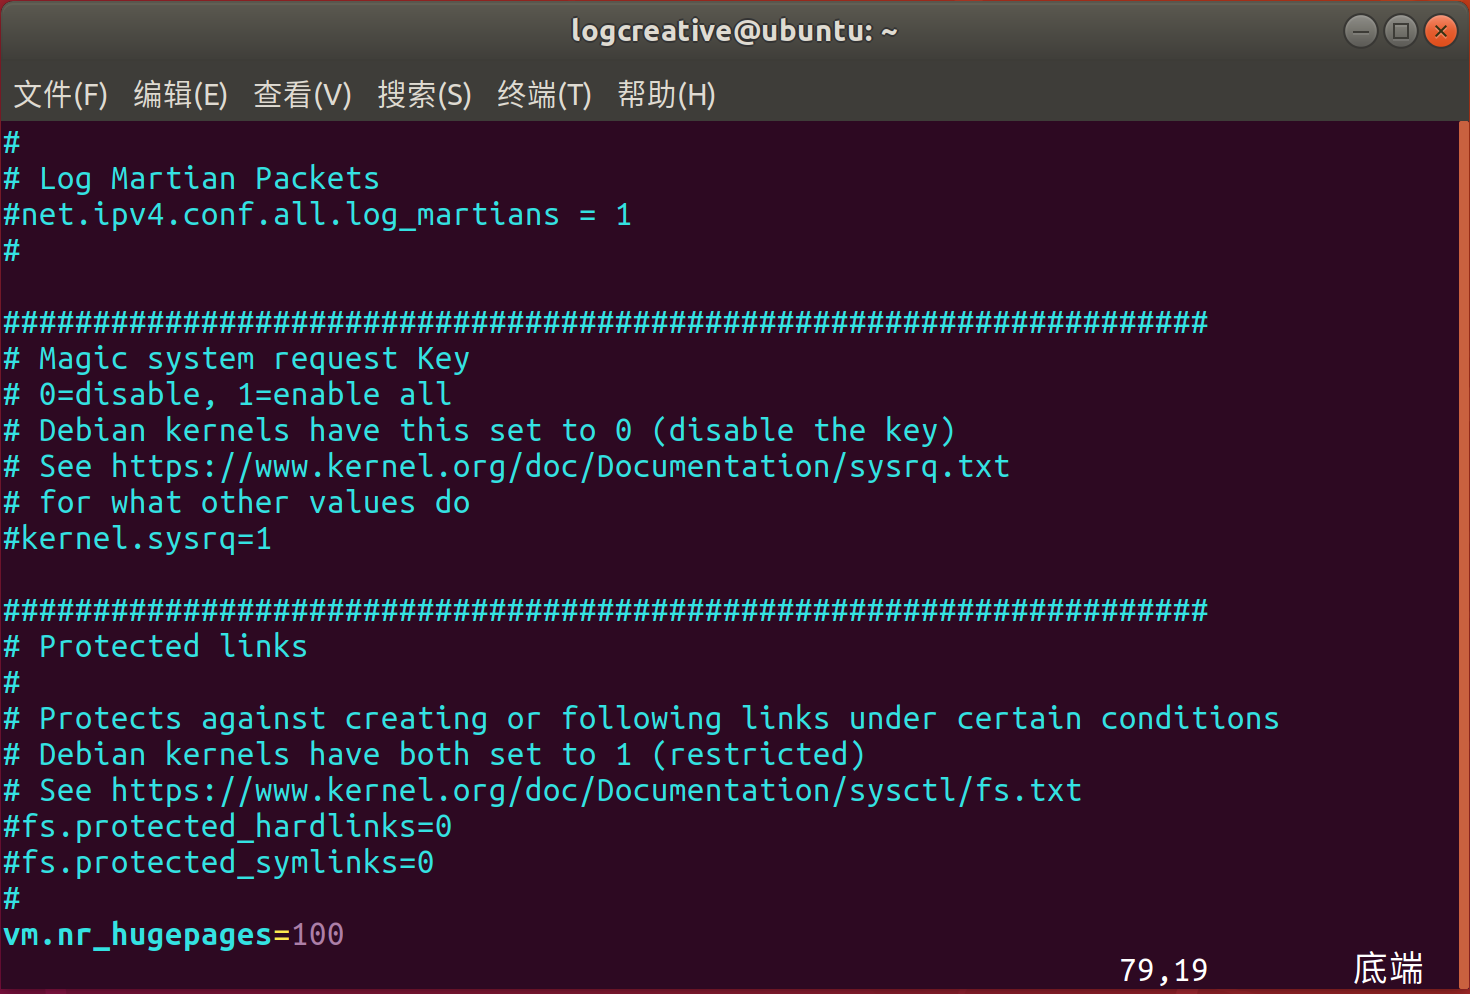
\includegraphics[width=0.95\linewidth]{confighugepage}
            \caption{配置大页}\label{fig:confighugepage}
        \end{minipage}
        \begin{minipage}{0.48\textwidth}
            \centering
            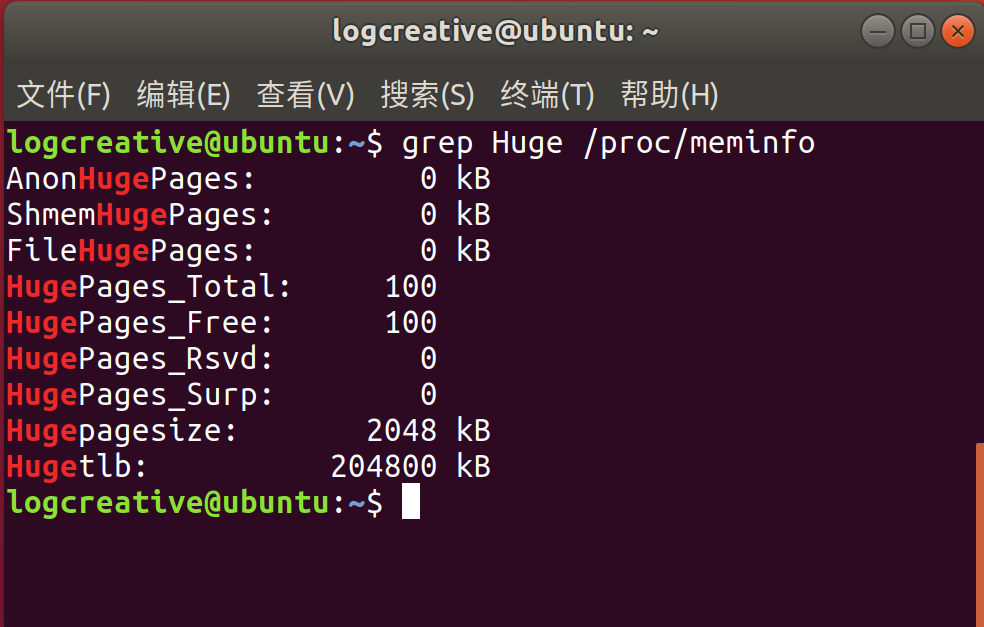
\includegraphics[width=\linewidth]{meminfo}
            \caption{显示配置}\label{fig:meminfo}
        \end{minipage}
    \end{figure}

    \section{创建对照虚拟机}

    在 \verb"virt-manager" 中克隆虚拟机,并在其中一个虚拟机中按照上述的方法配置大内存页。两种虚拟机都使用了 QEMU KVM。

    \begin{figure}[H]
        \centering
        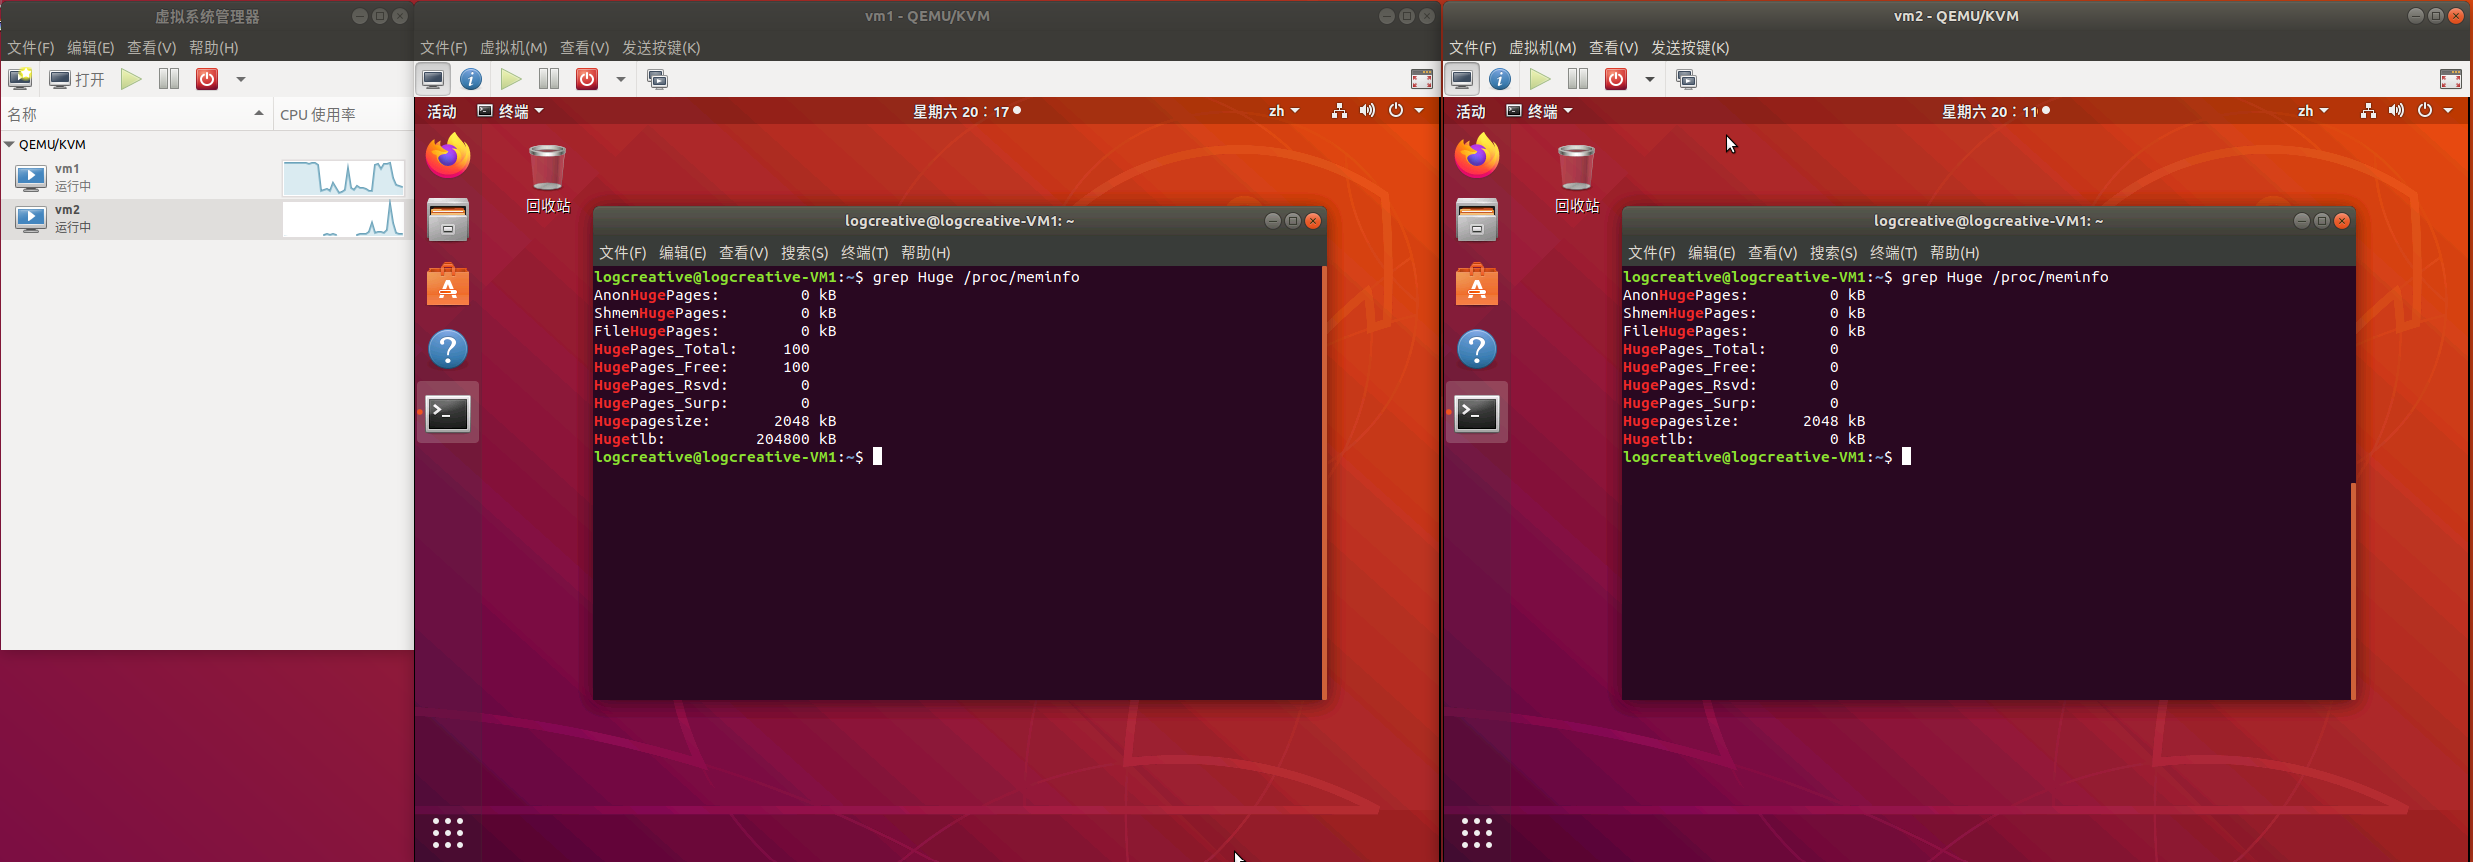
\includegraphics[width=\linewidth]{hugekvm}
        \caption{两种虚拟机}\label{fig:hugekvm}
    \end{figure}

    \section{运行测试}

    为了保证公平,测试仅运行于一个虚拟机开启的情况下。测试使用 \verb"sysbench"。
    
    \code[language=bash]{benchmark.sh}
    
    测试结果分别如图 \ref{fig:vm1} 和图 \ref{fig:vm2} 所示。

    \begin{figure}[H]
        \centering
        \begin{minipage}{0.48\textwidth}
            \centering
            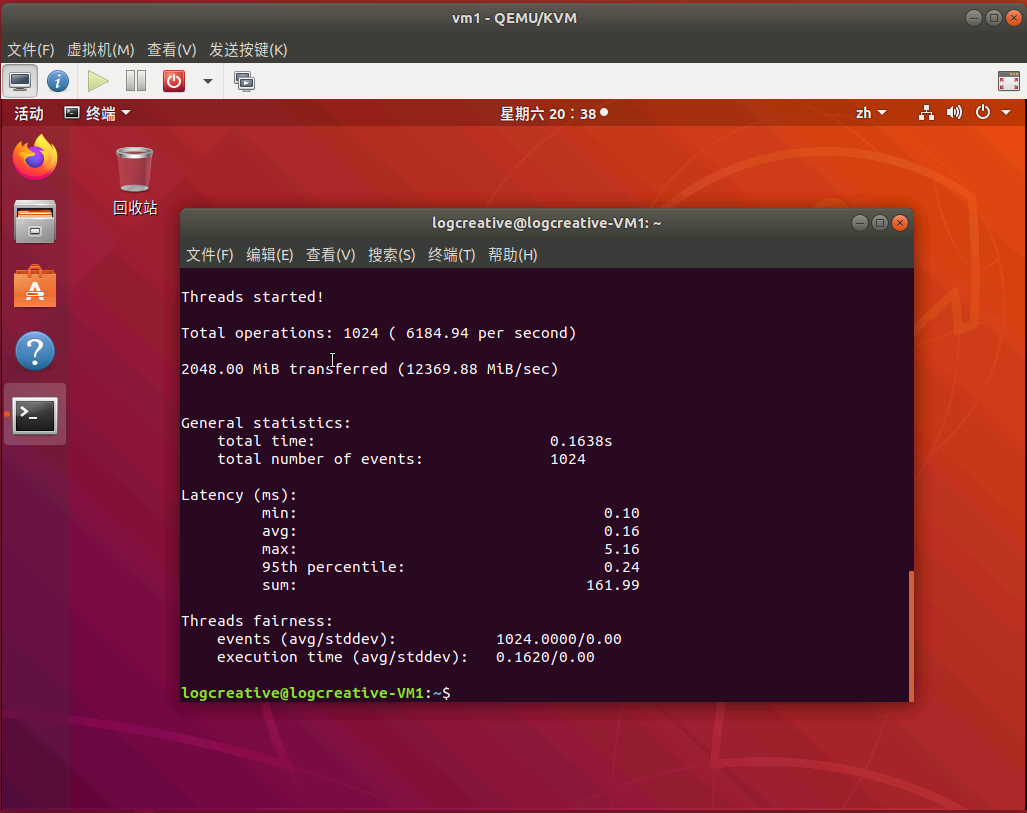
\includegraphics[width=\linewidth]{vm1}
            \caption{含有大内存页}\label{fig:vm1}
        \end{minipage}
        \begin{minipage}{0.48\textwidth}
            \centering
            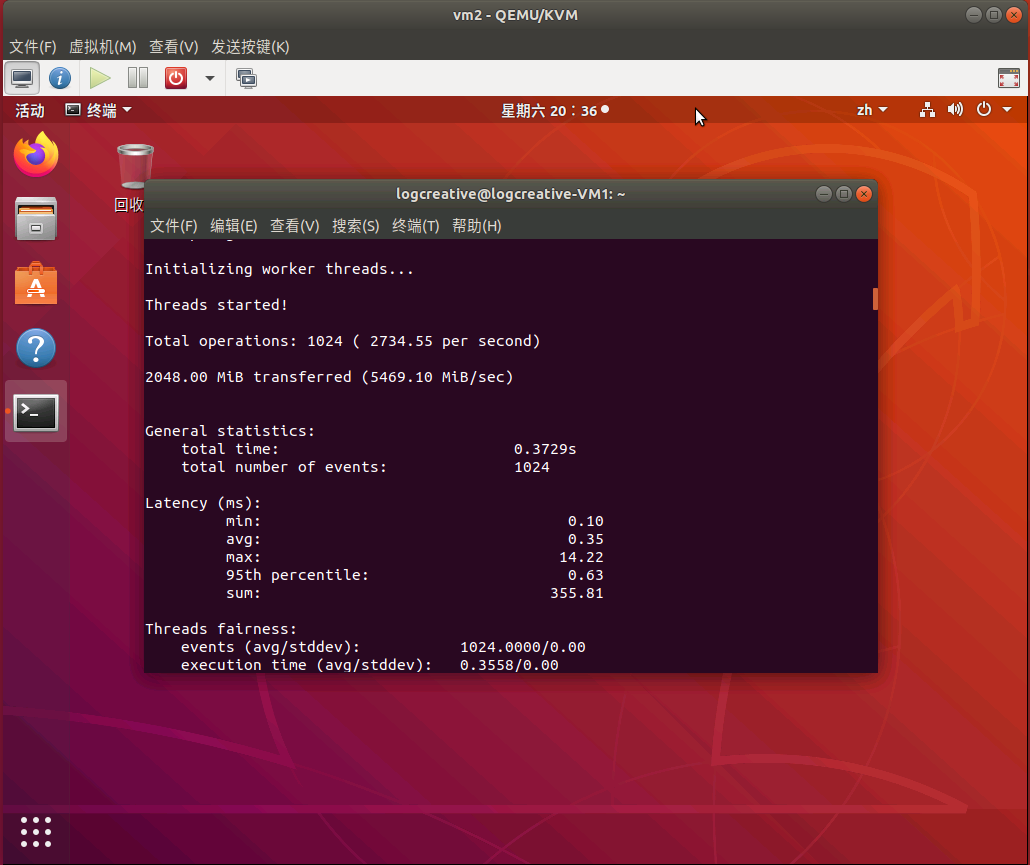
\includegraphics[width=0.95\linewidth]{vm2}
            \caption{不含有大内存页}\label{fig:vm2}
        \end{minipage}
    \end{figure}

    \section{解释}

    \begin{figure}[H]
        \centering
        \begin{minipage}{0.48\textwidth}
        \begin{tikzpicture}
            \begin{axis}[width=\linewidth,xlabel={Host},
            ymin={0},
            xmax={},
            ylabel={Total Time(s)},
            symbolic x coords={vm1,vm2}, xtick=data,
            ybar,enlarge x limits=0.8,]
             \addplot+ [] table[x=host,y=time,] {img/time.dat};
            \end{axis}
            \end{tikzpicture}            
        \caption{总时间比较}\label{fig:totaltime}
        \end{minipage}
        \begin{minipage}{0.48\textwidth}
        \begin{tikzpicture}
            \begin{axis}[width=\linewidth,legend pos={north west},
            xlabel={Host},
            ylabel={Latency (ms)},
            ymin={0},
            symbolic x coords={vm1,vm2}, xtick=data,
            ybar, enlarge x limits=0.8,]
             \pgfplotstableread [] {img/spec.dat}{\spec};
             \addplot+ [] table[x=host,y=min,] {\spec};
             \addplot+ [] table[x=host,y=avg,] {\spec};
             \addplot+ [] table[x=host,y=95,] {\spec};
             \legend{min,avg,95th,}
            \end{axis}
            \end{tikzpicture}  
            \caption{延迟比较}\label{fig:latency}
        \end{minipage}          
    \end{figure}

    由图 \ref{fig:totaltime} 可见,对于 2G 内存(2MB 块大小)写入测试上,开启了大内存页的 VM1 确实更占优势(降低了约 56\%),且在图 \ref{fig:latency} 的延迟比较上也占上风(总延迟降低了 54\%)。

    在虚拟内存管理中,内核维护一个将虚拟内存地址映射到物理地址的表,对于每个页面操作,内核都需要加载相关的映射。如果你的内存页很小,那么你需要加载的页就会很多,导致内核会加载更多的映射表。而这会降低性能。
    使用“大内存页”,意味着所需要的页变少了。从而大大减少由内核加载的映射表的数量。这提高了内核级别的性能最终有利于应用程序的性能。从而减少访问的开销。\cite{hugepage}

    而使用的大内存页都是 2M 的,并排布了 100 个,至少可以有效减少一部分内存页的访问开销,从而减少访问时间和延迟。

    \bibliography{ref}

\end{document}